% TODO:
% * List the feature functions that we use in our decoder.

\documentclass[11pt]{article}
%\usepackage{acl08}
\usepackage{acl-ijcnlp2009}
\usepackage{times}
\usepackage{latexsym}
\usepackage{multirow}
%\usepackage{clrscode}
\usepackage{amscd}
\usepackage{amsmath}
\usepackage{amssymb}
\usepackage{color}
\usepackage{epsfig}
\usepackage{float}
\usepackage{subfigure}
\usepackage{url}
\newcommand{\ignore}[1]{}


\title{Demonstration of Joshua: An Open Source Toolkit for Parsing-based Machine Translation\thanks{$\;\:$This
research was supported in part by the Defense Advanced Research Projects Agency's GALE program under
Contract No.\,HR0011-06-2-0001 and the National Science Foundation under grants No.\,0713448 and 0840112. The
views and findings are the authors' alone.}}

\author{
Zhifei Li,\,\,\,
Chris Callison-Burch,\,\,\, %add a footnote to mention that CCB is the project leader
Chris Dyer$^\dagger$,\,\,\,
Juri Ganitkevitch$^+$,\,\,\,
Sanjeev Khudanpur,\,\,\, \\
{\bf Lane Schwartz$^\star$,\,\,\,
Wren N.\,G.\,Thornton,\,\,\,
Jonathan Weese,\,\,
{\textnormal{and}}\,\,\,Omar F. Zaidan}\\
Center for Language and Speech Processing, Johns Hopkins University, Baltimore, MD\\
$\dagger$ Computational Linguistics and Information Processing Lab, University of Maryland, College Park, MD\\
$+$ Human Language Technology and Pattern Recognition Group, RWTH Aachen University, Germany\\
$\star$ Natural Language Processing Lab, University of Minnesota, Minneapolis, MN }


\date{}

\begin{document}

\maketitle


\begin{abstract}

We describe \textbf{Joshua} \cite{Joshua-WMT}\footnote{Please cite \newcite{Joshua-WMT} if you use
Joshua in your research, and {\bf not} this demonstration description paper.}, an open source toolkit for statistical machine
translation.  Joshua implements all of the algorithms required for translation
via synchronous context free grammars (SCFGs): chart-parsing, $n$-gram language
model integration, beam- and cube-pruning, and $k$-best extraction.  The toolkit
also implements suffix-array grammar extraction and minimum error rate training.
It uses parallel and distributed computing techniques for scalability.  We also
provide a demonstration outline for illustrating the toolkit's features to
potential users, whether they be newcomers to the field or power users interested
in extending the toolkit.

\end{abstract}

\section{Introduction}

Large scale parsing-based statistical machine translation (e.g., \newcite{Chiang2007},
\newcite{Quirk2005}, \newcite{Galley2006}, and \newcite{Liu2006}) has made
remarkable progress in the last few years.  However, most of the systems mentioned
above employ tailor-made, dedicated software that is not open source.  This results
in a high barrier to entry for other researchers, and makes experiments difficult to
duplicate and compare.  In this paper, we describe \textbf{Joshua}, a Java-based
general-purpose open source toolkit for parsing-based machine translation, serving the
same role as Moses \cite{Moses} does for regular phrase-based machine translation.

%Our toolkit is written in Java and implements all the essential algorithms described
%in \newcite{Chiang2007}: chart-parsing, $n$-gram language model integration, beam-
%and cube-pruning, and $k$-best extraction.  The toolkit also implements suffix-array
%grammar extraction \cite{Lopez2007} and minimum error rate training \cite{Och2003c}.
%Additionally, parallel and distributed computing techniques are exploited to make it
%scalable \cite{Li2008b}. We have also made great effort to ensure that our toolkit
%is easy to use and to extend.

%\textbf{TODO: adapt concluding paragraph? WMT09 results?}

%The toolkit has been used to translate roughly a million sentences in a parallel
%corpus for large-scale discriminative training experiments \cite{Li2008}.
%The decoder has also been successfully used by other researchers. For example,
%\newcite{sg-boxing} have demonstrated that our decoder achieves performance
%competitive with Moses \cite{Moses}.
%We hope the release of the toolkit will greatly contribute the progress of the
%syntax-based machine translation research.\footnote{The toolkit can be downloaded
%at \url{http://www.sourceforge.net/projects/joshua}, and the instructions in
%using the toolkit are at \url{http://cs.jhu.edu/~ccb/joshua}.}

\section{Joshua Toolkit}
When designing our toolkit, we applied general principles of software engineering
to achieve three major goals: \emph{Extensibility}, \emph{end-to-end coherence},
and \emph{scalability}.

\textbf{Extensibility:} Joshua's codebase consists of a separate Java \texttt{package}
for each major aspect of functionality.  This way, researchers can focus on a single \texttt{package}
of their choosing.  Fuurthermore, extensible components are defined by Java
\texttt{interface}s to minimize unintended interactions and unseen dependencies, a common hindrance to
extensibility in large projects.  Where there is a clear point of departure for research, a basic
implementation of each \texttt{interface} is provided as an \texttt{abstract class} to minimize
work necessary for extensions.

\textbf{End-to-end Cohesion:} An MT pipeline consists of many diverse components,
often designed by separate groups that have different file formats and interaction requirements.
This leads to a large number of scripts for format conversion and to facilitate interaction
between the components, resulting in untenable
and non-portable projects, and hindering repeatability of experiments.  Joshua, on the
other hand, integrates the critical components of an MT pipeline seamlessly.
Still, each component can be used as a stand-alone tool that does not rely on the rest of the toolkit.

\textbf{Scalability}: Joshua, especially the decoder, is scalable
to large models and data sets. For example, the parsing and pruning algorithms are
implemented with dynamic programming strategies and efficient data structures. We also
utilize suffix-array grammar extraction, parallel/distributed decoding, and bloom filter
language models.

Joshua offers state-of-the-art quality, having been
ranked 4th out of 16 systems in the French-English task of the 2009 WMT
evaluation, both in automatic (Table~\ref{results-wmt09}) and human
evaluation.

\begin{table}[t]
\begin{center}
\begin{tabular}{c c}\hline
  System & B{\small LEU}-4 \\ \hline
  google & 31.14 \\
  lium & 26.89 \\
  dcu & 26.86 \\
  {\bf joshua} & {\bf 26.52} \\
  uka & 25.96 \\
  limsi & 25.51 \\
  uedin & 25.44 \\
  rwth & 24.89 \\
  cmu-statxfer & 23.65 \\ \hline
\end{tabular}
\end{center}
\caption{B{\small LEU} scores for top primary systems on the WMT-09 French-English Task from \newcite{WMT09-Findings},
who also provide human evaluation results.}
\label{results-wmt09}
\end{table}

\subsection{Joshua Toolkit Features}

Here is a short description of Joshua's main features, described in more detail in \newcite{Joshua-WMT}:

\begin{itemize}
\item \textbf{Training Corpus Sub-sampling:} We support inducing a grammar from
a subset of the training data, that consists of sentences needed to translate a particular
test set.  To accomplish this, we make use of the method proposed by Kishore
Papineni (personal communication), outlined in further detail in \cite{Joshua-WMT}.
The method achieves a 90\% reduction in training
corpus size while maintaining state-of-the-art performance.

% to. This method works as follows: for the development and test sets that will be
%translated, every $n$-gram (up to length 10) is gathered into a map $\mathcal{W}$
%and associated with an initial count of zero.  Proceeding in order through the
%training data, for each sentence pair whose source-to-target length ratio is within
%one standard deviation of the average, if any $n$-gram found in the \emph{source sentence}
%is also found in $\mathcal{W}$ with a count of less than $k$, the sentence is selected.
%When a sentence is selected, the count of every $n$-gram in $\mathcal{W}$ that is found
%in the source sentence is incremented by the number of its occurrences in the source
%sentence. \ignore{Thus, there are two conditions in which a sentence will not be
%selected: 1) it only contains $n$-grams that are not found in $\mathcal{W}$ (making
%it useless for learning in the highly lexicalized models we use) or 2) it only
%contains $n$-grams that have already been attested in the selected set $k$ or more
%times.} For our submission, we used $k=20$, which resulted in 1.5 million (out of
%23 million) sentence pairs being selected for use as training data.  There were
%30,037,600 English words and 30,083,927 French words in the subsampled training corpus.

\item \textbf{Suffix-array Grammar Extraction:}
Grammars extracted from large training corpora are often far too large to fit
into available memory.
Instead, we follow \newcite{Callison-Burch2005b} and \newcite{Lopez2007}, and
use a source language suffix array to extract only rules that will actually be
used in translating a particular test set.
Direct access to the suffix array is incorporated into the decoder, allowing
rule extraction to be performed for each input sentence individually, but
it can also be executed as a standalone pre-processing step.

\item \textbf{Grammar formalism:} Our decoder assumes a probabilistic synchronous
context-free grammar (SCFG). It handles SCFGs of the kind extracted
by Hiero \cite{Chiang2007}, but is easily extensible to more general SCFGs (as in
\newcite{Galley2006}) and closely related formalisms like synchronous tree
substitution grammars \cite{Eisner2003}.

%\item \textbf{Chart parsing:} Given a source sentence to decode, the decoder generates
%a one-best or $k$-best translations using the CKY algorithm.

\item \textbf{Pruning:} We incorporate beam- and cube-pruning \cite{Chiang2007}
to make decoding feasible for large SCFGs.

\item \textbf{$k$-best extraction:}
Given a source sentence, the chart-parsing algorithm produces a \emph{hypergraph}
representing an exponential number of derivation hypotheses.  We implement the
extraction algorithm of \newcite{Huang2005} to extract the $k$ most likely
derivations from the hypergraph.

\item \textbf{Oracle Extraction:}
Even within the large set of translations represented by a hypergraph,
some desired translations (e.g. the references)
may not be contained due to pruning or inherent modeling deficiency.
We implement an efficient dynamic programming algorithm \cite{oracleExtraction2009}
for finding the \emph{oracle translations}, which are most similar to the desired translations, as measured by
a metric such as B{\small LEU}.

\item \textbf{Parallel and distributed decoding:}
We support \emph{parallel decoding} and a \emph{distributed language model}
that exploit multi-core and multi-processor architectures and distributed computing
\cite{Li2008b}.

\item \textbf{Language Models:} We implement three local $n$-gram language models:
a straightforward implementation of the $n$-gram scoring function in Java, capable
of reading standard ARPA backoff $n$-gram models;
a native code bridge that allows the decoder to use the SRILM toolkit to
read and score $n$-grams\footnote{The first implementation
allows users to easily try the Joshua toolkit without installing SRILM.
However, users should note that the
basic Java LM implementation is not as scalable as the SRILM native bridge code.};
and finally a Bloom Filter implementation following \newcite{Talbot2007a}.

\item \textbf{Minimum Error Rate Training:} Joshua's MERT module optimizes parameter
weights so as to maximize performance on a development set as measured by an automatic
evaluation metric, such as B{\small LEU}.  The optimization consists of a series of
line-optimizations using the efficient method of \newcite{Och2003c}.  More details on the MERT method
and the implementation can be found in \newcite{Zaidan2009forwmt}.\footnote{The module
is also available as a standalone application, {\em Z-MERT}, that can be used with other
MT systems.  (Software and documentation at: \url{http://cs.jhu.edu/~ozaidan/zmert}.)}

\item \textbf{Variational Decoding:} \emph{spurious ambiguity} causes the probability of
an output string among to be split among many derivations.  The goodness
of a string is measured by the total probability of its derivations, which means
that finding the best output string is computationally intractable.
The standard Viterbi approximation is based on the most probable derivation, but
we also implement a variational approximation, which considers all the derivations
but still allows tractable decoding \cite{Li2009}.
\end{itemize}

\section{Demonstration Outline}

The purpose of the demonstration is 4-fold: 1) to give newcomers to the field
of statistical machine translation an idea of the state-of-the-art; 2) to show
actual, live, end-to-end operation of the system,
highlighting its main components, targeting potential users; 3) to illustrate,
through visual aids, the underlying algorithms, for those interested in the
technical details; and 4) to explain how those components can be extended, for
potential \emph{power users} who want to be familiar with the code itself.

The first component of the demonstration will be an interactive user interface,
where arbitrary user input in a source language is entered into a web form and
then translated into a target language by the system.  This component
specifically targets newcomers to SMT, and demonstrates the current state of
the art in the field.  We will have trained multiple systems (for multiple
language pairs), hosted on a remote server, which will be queried with the
sample source sentences.

Potential users of the system would be interested in seeing an actual operation
of the system, in a similar fashion to what they would observe on their own
machines when using the toolkit.  For this purpose, we will demonstrate three
main modules of the toolkit: the rule extraction module, the MERT module, and
the decoding module.  Each module will have a separate terminal window
executing it, hence demonstrating both the module's expected output as well as
its speed of operation.

In addition to demonstrating the functionality of each module, we will also
provide accompanying visual aids that illustrate the underlying algorithms and
the technical operational details.  We will provide visualization of the search
graph and the 1-best derivation, which would illustrate the functionality of
the decoder, as well as alternative translations for phrases of the source
sentence, and where they were learned in the parallel corpus, illustrating the
functionality of the grammar rule extraction.  For the MERT module, we will
provide figures that illustrate Och's efficient line search method.

%Finally, power users of the system would be interested in extending the toolkit
%to accommodate new functionality.  To that end, we will specifically illustrate
%several potential extensions to the toolkit by highlighting portions of the
%code that the user would be expected to modify and/or augment when implementing
%such extensions.  For instance, we will point out how a new feature function
%can be added to the decoder, or how a new metric can be incorporated to the
%MERT module.

\section{Demonstration Requirements}

The different components of the demonstration will be spread across at most 3
machines (Figure~\ref{fig:setup}): one for the live ``instant translation'' user interface, one for
demonstrating the different components of the system and algorithmic
visualizations, and one designated for technical discussion of the code.  We
will provide the machines ourselves and ensure the proper software is installed
and configured.  However, we are requesting that large LCD monitors be made
available, if possible, since that would allow more space to demonstrate the
different components with clarity than our laptop displays would provide.  We
will also require Internet connectivity for the live demonstration, in order to
gain access to remote servers where trained models will be hosted.

\begin{figure*}[t]
\begin{centering}
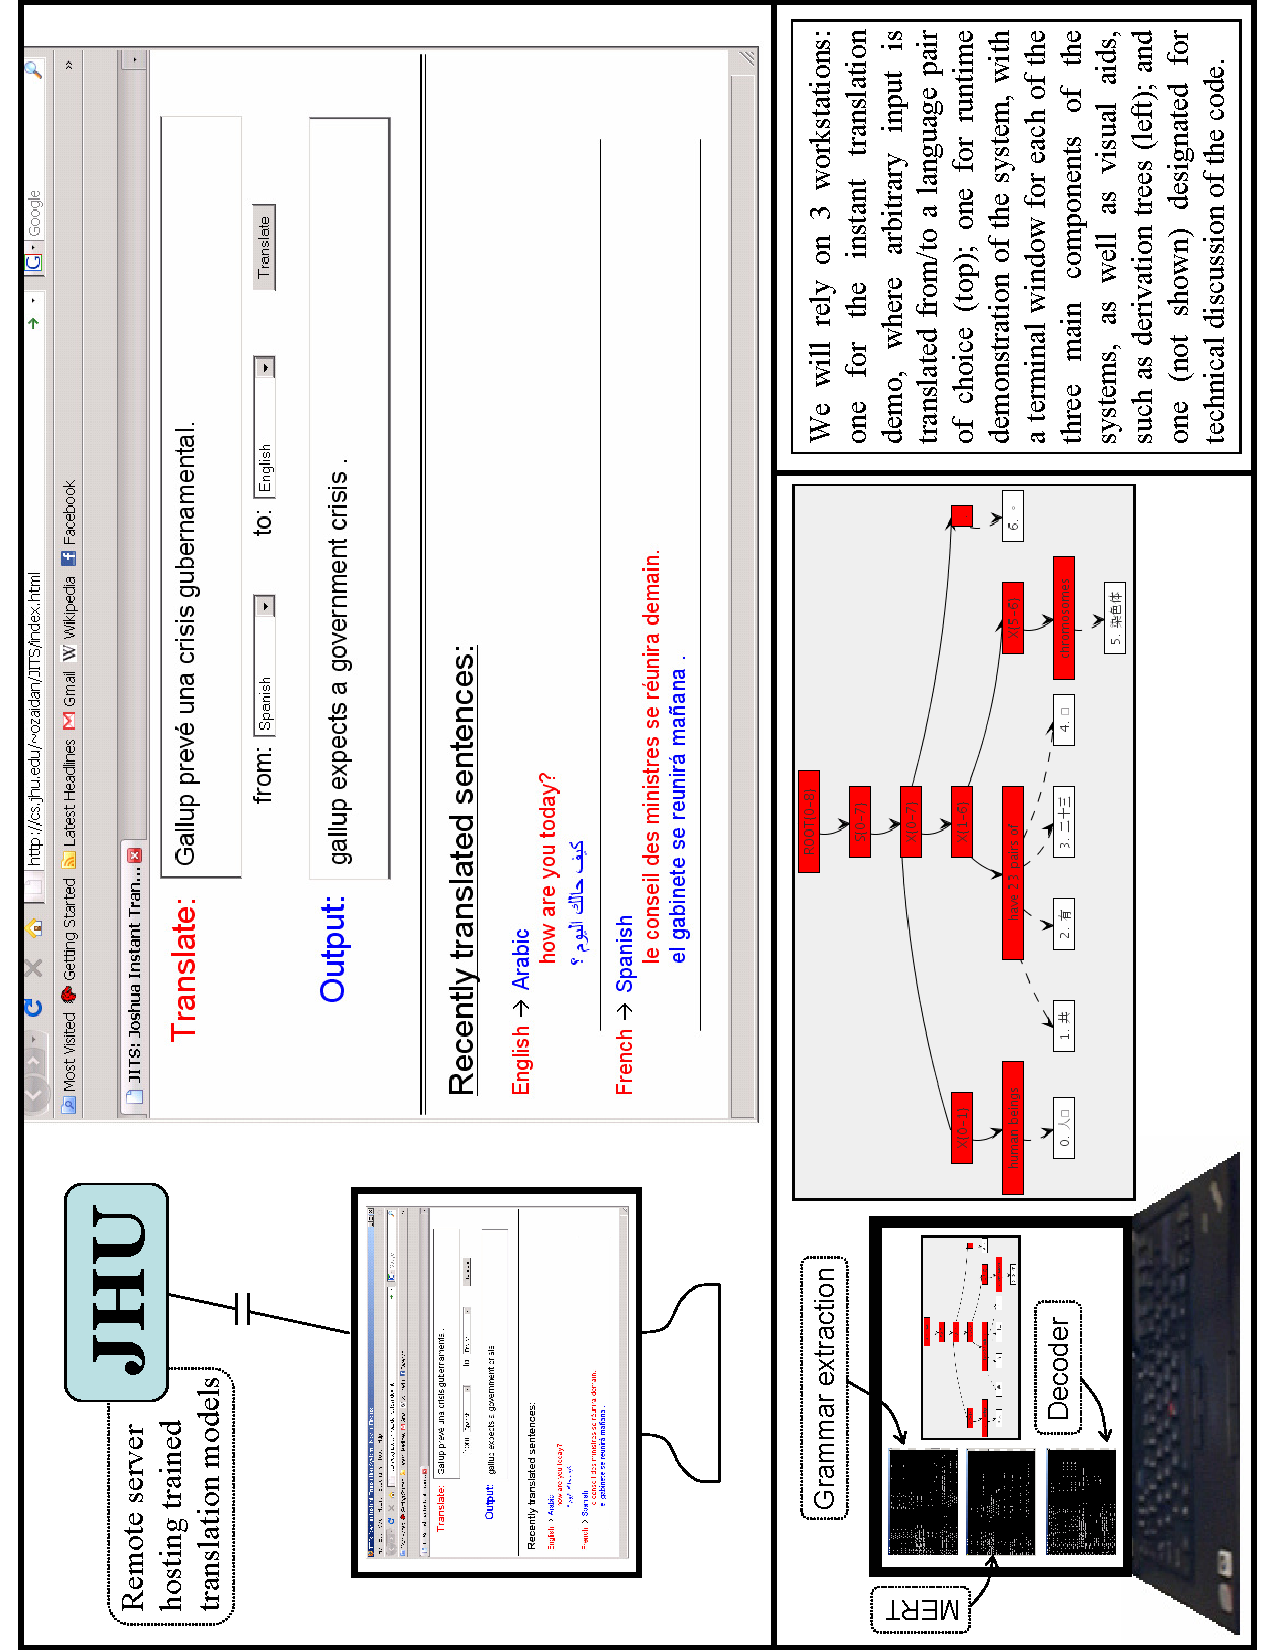
\includegraphics[scale=0.57,angle=270]{demo-setup.pdf}
\caption{Proposed setup of our demonstration. When this paper is viewed as a PDF, the reader
may zoom in further to see more details.}
\label{fig:setup}
\end{centering}
\end{figure*}

%%%lzf add this section

%%%%%%%%%%%%%%%%%%%%%%%%%%%%%%%%%%%%%%%%%%%%%%%%%%%%%

%\section*{Acknowledgments}
%This research was supported in part by the Defense Advanced Research Projects Agency's GALE program under Contract No.\,HR0011-06-2-0001 and the National Science Foundation under grants No.\,0713448 and 0840112. The views and findings are the authors' alone.

%%%%%%%%%%%%%%%%%%%%%%%%%%%%%%%%%%%%%%%%%%%%%%%%%%%%%

\bibliographystyle{acl}
\bibliography{../bibliography}
\end{document}
